\documentclass[11pt]{beamer}
\usepackage{listings} % Include the listings-package
\usepackage[T1]{fontenc}
\usepackage[utf8]{inputenc}
\usepackage[english]{babel}
\usepackage{amsmath}
\usepackage{amssymb, amsfonts, latexsym, cancel}
\usepackage{float}
\usepackage{graphicx}
\usepackage{epstopdf}
\usepackage{subfigure}
\usepackage{hyperref}
\usepackage{indentfirst}
%\usepackage{authblk}
\usepackage{blindtext}
\usepackage{booktabs} % Allows the use of \toprule, 
\usepackage{filecontents}
\usepackage{courier} %% Sets font for listing as Courier.
\usepackage{listings}
\usepackage{ragged2e}
\usepackage{listings, xcolor}
%\usepackage{parskip}
%\usepackage[margin=10cm]{geometry}
\lstset{
tabsize = 2, %% set tab space width
showstringspaces = false, %% prevent space marking in strings, string is defined as the text that is generally printed directly to the console
numbers = left, %% display line numbers on the left
commentstyle = \color{green}, %% set comment color
keywordstyle = \color{blue}, %% set keyword color
stringstyle = \color{red}, %% set string color
rulecolor = \color{black}, %% set frame color to avoid being affected by text color
basicstyle = \small \ttfamily , %% set listing font and size
breaklines = true, %% enable line breaking
numberstyle = \tiny,
}
\usepackage{caption}
\DeclareCaptionFont{white}{\color{white}}
\DeclareCaptionFormat{listing}{\colorbox{gray}{\parbox{\textwidth}{#1#2#3}}}
\captionsetup[lstlisting]{format=listing,labelfont=white,textfont=white}
\definecolor{urlColor}{rgb}{0.06, 0.3, 0.57}
\definecolor{linkColor}{rgb}{0.57, 0.0, 0.04}
\definecolor{fileColor}{rgb}{0.0, 0.26, 0.26}
\hypersetup{
    colorlinks=true,
    linkcolor=linkColor,
    filecolor=fileColor,      
    urlcolor=urlColor,
}
\urlstyle{same}
\setbeamercovered{transparent}
%\usetheme{Boadilla}
\usetheme{CambridgeUS}
%\usetheme{Berkeley}
%\usetheme{Warsaw}
%\usetheme{Madrid}

\title[Introducción]{\bf\Huge Johnson (2007)}
\subtitle{Interacción Humano Computador}

\author[Grupo 10]
{
    Deyson Victor Diaz Ticona, 
    Kevin Yunior Ccorimanya Paucar, 
    Denilson Flores Valdivia,
    Marco Antonio Ponce de Leon 
}
\institute[UNSA]
{
System Engineering School\\
System Engineering and Informatic Department\\
Production and Services Faculty\\
San Agustin National University of Arequipa
}

\date[2020-09-16]{\scriptsize{2020-09-16}}
%\logo{
\includegraphics[width=3.0cm]{logo_unsa.jpg}}
\titlegraphic{
\includegraphics[width=1.0cm]{logo_unsa.jpg}}

\begin{document}

\begin{frame}
\titlepage
\end{frame}

\begin{frame}
\frametitle{Content}
\tableofcontents
\end{frame}

\section{Analisis de Tareas}
\begin{frame}

\frametitle{Analisis de Tareas}
\par
\justify
\color{black}
Describir en detalle cómo analizar los objetivos y tareas de los usuarios. Entonces, un buen análisis de tareas responde a las siguientes preguntas:
\begin{itemize}
    \item ¿Qué objetivos quieren alcanzar los usuarios al utilizar la aplicación?
    \item ¿Qué conjunto de tareas humanas pretende admitir la aplicación?
    \item ¿Qué tareas son más importantes y cuáles son las menos importantes?
    \item ¿Cuáles son los pasos de cada tarea?
    \item ¿Cuáles son el resultado y el producto de cada tarea?
    \item ¿De dónde proviene la información de cada tarea?
    \item ¿Cómo se utiliza la información que resulta de cada tarea?
    \item ¿Qué herramientas se utilizan para realizar cada tarea?
    \item ¿Qué problemas tienen las personas para realizar cada tarea? ¿Qué tipo de errores son comunes? ¿Qué los causa? ¿Qué tan dañinos son los errores?
\end{itemize}
\end{frame}

\begin{frame}
\frametitle{Analisis de Tareas}
    \par
    \justify
    \color{black}
    Una vez que se responden estas preguntas, el siguiente paso es comenzar a dibujar posibles interfaces de usuario. Luego tenemos que diseñar un modelo conceptual para la herramienta que se centra en las tareas y objetivos de los usuarios. Después de haber diseñado un modelo conceptual centrado en tareas, tan simple y consistente posible, podemos diseñar una interfaz de usuario que minimiza el tiempo y la experiencia necesarios para utilizar la aplicación y asi convertirse en un proceso automático.
    \begin{figure}
    \centering
     
\includegraphics[width=0.3\textwidth]{imagen9.jpg} 
    \end{figure}
\end{frame}

\section{Principios de Interaccion Humano - Computador}
\begin{frame}
\frametitle{Principios de Interaccion Humano - Computador}
\begin{itemize}
    \item Principio 1: Centrarse en los usuarios y sus tareas, no en la tecnología
    \item Principio 2: Considere la función primero, la presentación después
    \item Principio 3: Conforme a la visión de la tarea de los usuarios
    \item Principio 4: Diseño para el caso común
    \item Principio 5: No complique la tarea de los usuarios
    \item Principio 6: Facilitar el aprendizaje
    \item Principio 7: Entregue información, no solo datos
    \item Principio 8: Diseño para la capacidad de respuesta
    \item Principio 9: Pruébelo con los usuarios; entonces arréglalo
\end{itemize}
\end{frame}


\begin{frame}
\frametitle{Principio 1: Centrarse en los usuarios y sus tareas, no en la tecnología}
    \par
    \justify
    \color{black}
    \begin{itemize}
    \item Entender a los usuarios
    \item Entender las tareas
    \item Considere el contexto en el que funcionará el software
    \end{itemize}
    \par
    \vspace{2mm}
    Para un correcto cumplimiento de los objetivos, la tecnología toma un lugar secundario y se prioriza el entendimiento del usuario y la eficacia del sistema.
    \begin{figure}
    \centering
     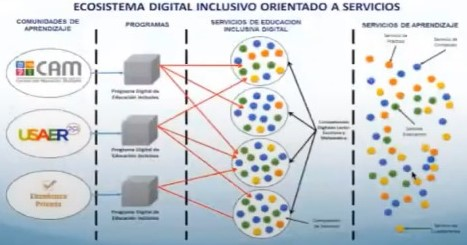
\includegraphics[width=0.4\textwidth]{imagen8.jpg} 
    \end{figure}
\end{frame}

\begin{frame}
\frametitle{Principio 2: Considere la función primero, la presentación después}
    \par
    \justify
    \color{black}
    \begin{itemize}
    \item Desarrollar un modelo conceptual que cumple de manera completa el objetivo del mismo.
    \end{itemize}
    \par
    \vspace{2mm}
    El cumplimiento de la tarea siempre será la prioridad.
    \begin{figure}
    \centering
     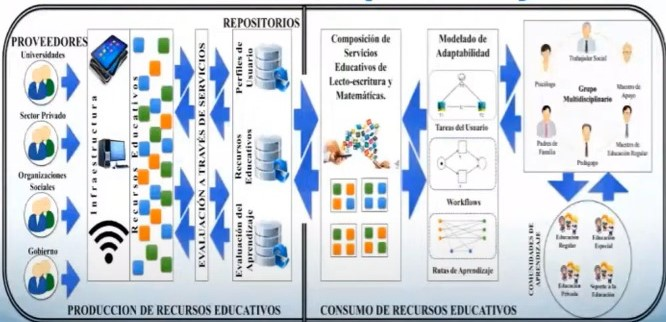
\includegraphics[width=0.4\textwidth]{imagen7.jpg} 
    \end{figure}
\end{frame}

\begin{frame}
\frametitle{Principio 3: Conforme a la visión de la tarea de los usuarios}
    \par
    \justify
    \color{black}
    \begin{itemize}
    \item Lucha por la naturalidad
    \item Utilice el vocabulario de los usuarios, no el suyo
    \item Mantenga los componentes internos del programa dentro del programa
    \item Encuentre el punto correcto sobre el equilibrio entre potencia y complejidad
    \end{itemize}
    \par
    \vspace{2mm}
    Para poder brindar algo optimo, el lenguaje a utilizar para los usuarios debe ser lo más simple posible, no resultar forzado para ellos, y debe ser sencilla y práctica.
    \begin{figure}
    \centering
     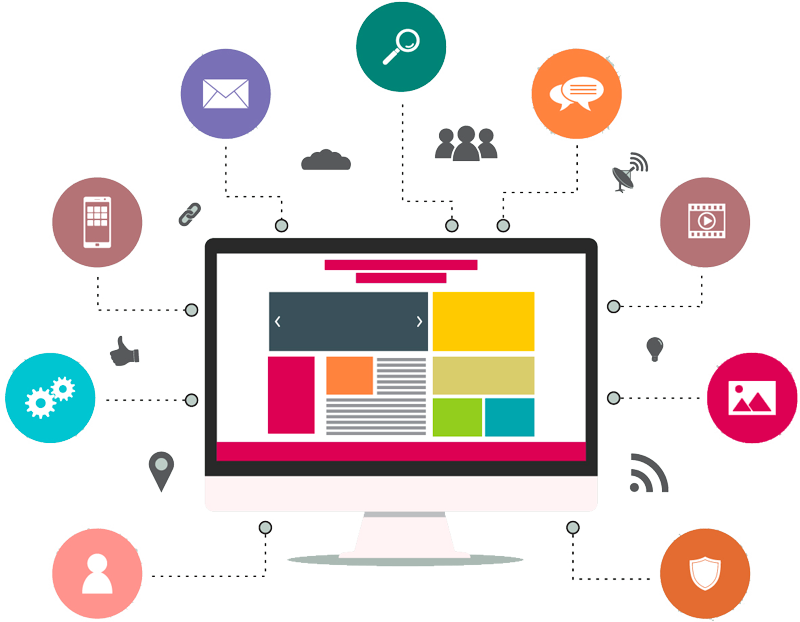
\includegraphics[width=0.3\textwidth]{imagen6.png} 
    \end{figure}
\end{frame}

\begin{frame}
\frametitle{Principio 4: Diseño para el caso común}
    \par
    \justify
    \color{black}
    \begin{itemize}
    \item Hacer que los resultados comunes sean fáciles de lograr
    \item Dos tipos de "comunes": "cuántos usuarios" y "con qué frecuencia"
    \item Diseño para casos básicos; no te preocupes por los casos de "borde"
    \end{itemize}
    \par
    \vspace{2mm}
    Como ya se mencionó, la practicidad y el nivel de interacción deben ser simples y prácticos para el entendimiento e interacción del usuario.
    \begin{figure}
    \centering
     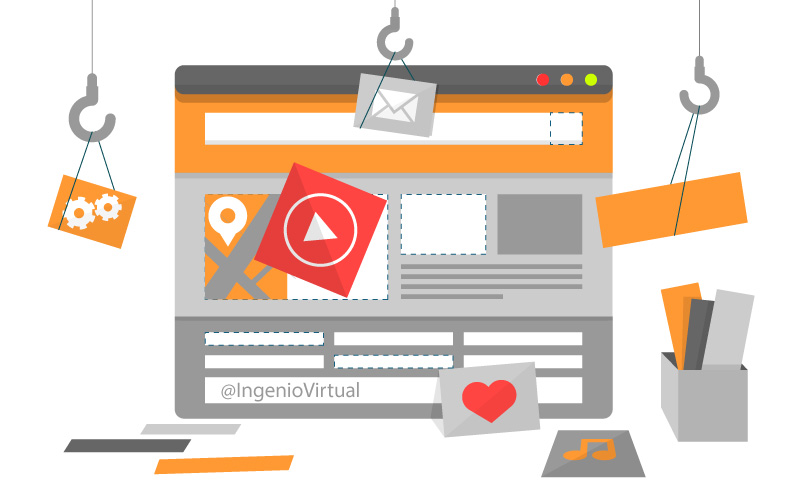
\includegraphics[width=0.4\textwidth]{imagen5.jpg} 
    \end{figure}
\end{frame}

\begin{frame}
\frametitle{Principio 5: No complique la tarea de los usuarios}
    \par
    \justify
    \color{black}
    \begin{itemize}
    \item No les dé problemas adicionales a los usuarios
    \item No hagas que los usuarios razonen por eliminación
    \end{itemize}
    \par
    \vspace{2mm}
    Para el usuario, debe ser sencillo interactuar con el sistema, por esa razón las tareas que se le proporciona deben ser claras y exactas, no interponer varias acciones o tareas que puedan confundir a los usuarios.
    \begin{figure}
    \centering
     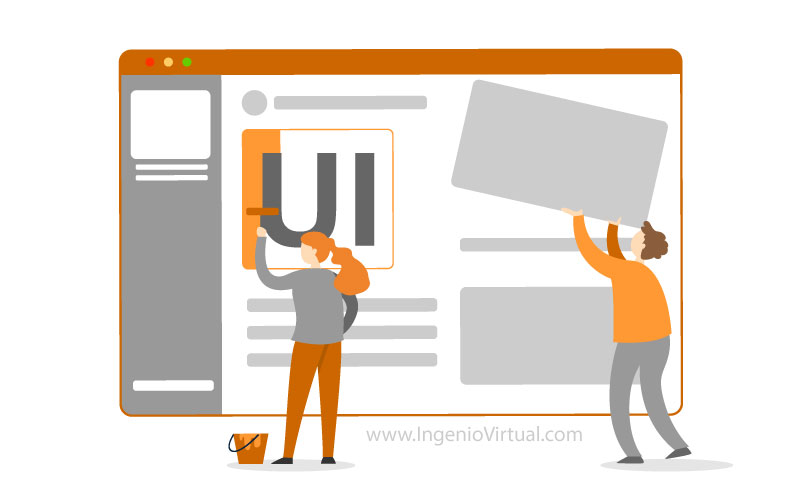
\includegraphics[width=0.4\textwidth]{imagen4.jpg} 
    \end{figure}
\end{frame}

\begin{frame}
\frametitle{Principio 6: Facilitar el aprendizaje}
    \par
    \justify
    \color{black}
    \begin{itemize}
    \item Piense "de afuera hacia adentro", no "de adentro hacia afuera"
    \item Consistencia, consistencia, consistencia 
    \item Proporcionar un entorno de bajo riesgo
    \end{itemize}
    \par
    \vspace{2mm}
    Para el que interacciona, las tareas asignadas deben ser simples, que no comprometan la funcionalidad del sistema.
    \begin{figure}
    \centering
     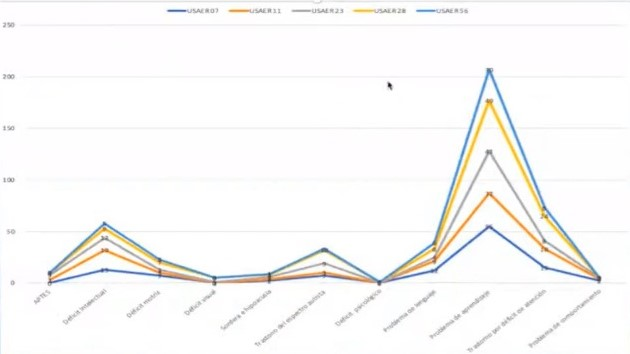
\includegraphics[width=0.3\textwidth]{imagen3.jpg} 
    \end{figure}
\end{frame}

\begin{frame}
\frametitle{Principio 7: Entregue información, no solo datos}
    \par
    \justify
    \color{black}
    \begin{itemize}
    \item Diseñe las exhibiciones cuidadosamente; conseguir ayuda profesional
    \item La pantalla pertenece al usuario 
    \item Preservar la inercia de la pantalla 
    \end{itemize}
    \begin{figure}
    \centering
     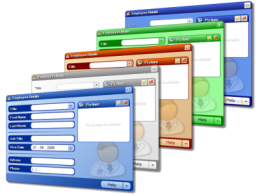
\includegraphics[width=0.3\textwidth]{imagen2.png} 
    \end{figure}
\end{frame}

\begin{frame}
\frametitle{Principio 8: Diseño para la capacidad de respuesta}
    \par
    \justify
    \color{black}
    \begin{itemize}
    \item Reconocer las acciones del usuario al instante 
    \item Informar a los usuarios cuando el software está ocupado y cuando no 
    \item Libera a los usuarios para que hagan otras cosas mientras esperan 
    \item Animar el movimiento de forma suave y clara 
    \item Permitir a los usuarios abortar operaciones prolongadas que no desean
    \item Permitir a los usuarios estimar cuánto tiempo tomarán las operaciones
    \item Trate de permitir que los usuarios establezcan su propio ritmo de trabajo
    \end{itemize}
    \par
    \vspace{2mm}
    Para el usuario, las acciones deben ser comprensibles, para esto, la información que se le brinda debe estar a un nivel simple de entendimiento, con una retroalimentación moderada, y poder darle la opción de cancelar y medir el proceso de trabajo.
\end{frame}

\begin{frame}
\frametitle{Principio 9: Pruébelo con los usuarios; entonces arréglalo}
    \par
    \justify
    \color{black}
    \begin{itemize}
    \item Los resultados de las pruebas pueden sorprender incluso a los         diseñadores experimentados 
    \item Programe tiempo para corregir los problemas encontrados por las pruebas
    \item Las pruebas tienen dos objetivos: informativos y sociales.
    \item Hay pruebas para cada momento y propósito
    \end{itemize}
    \begin{figure}
    \centering
     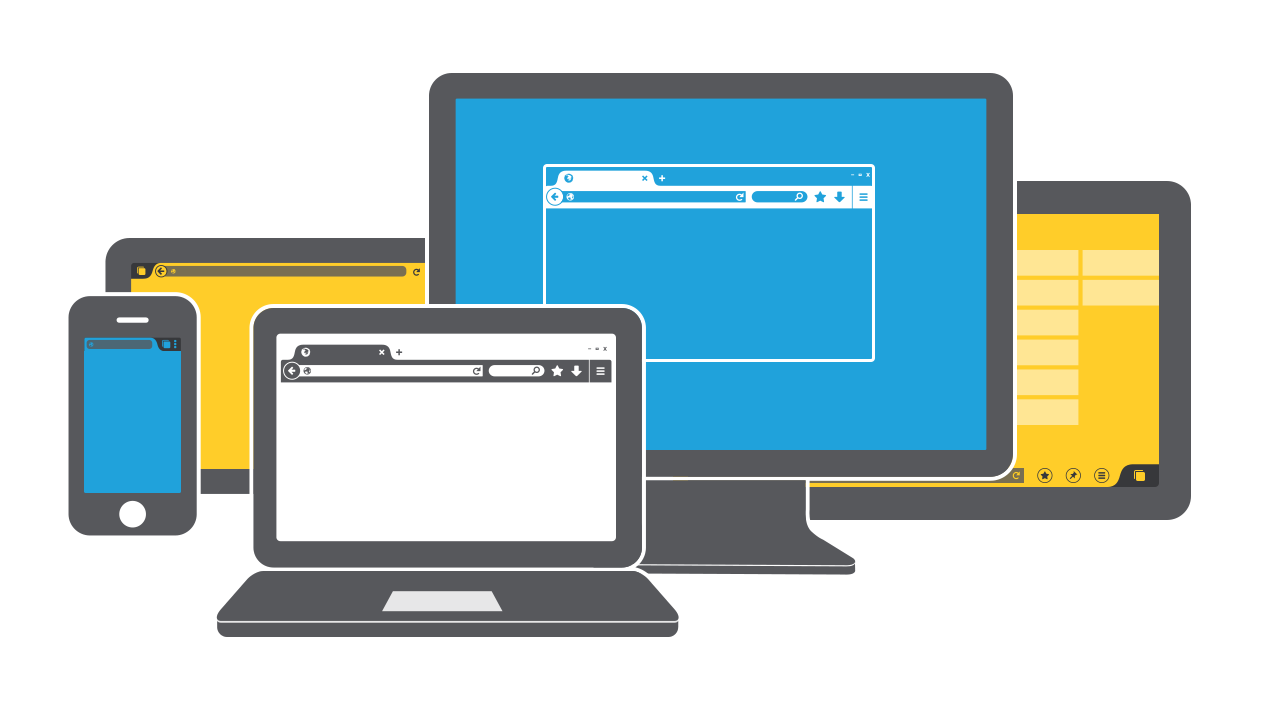
\includegraphics[width=0.4\textwidth]{imagen.png} 
    \end{figure}
\end{frame}

\section{References}
%References frame
\begin{frame}
\frametitle{References}
\begin{itemize}
\item Introduction - xiii, Jhonson J. (2014). Designing with the Mind in mind. 2nd. edition.
\end{itemize}
\end{frame}

\end{document}